%!TEX root = ../main.tex
%%%%%%%%%%%%%%%%%%%%%%%%%%%%%%%%%%
% Links:
%
% Difficulty:
% Companies: 
%%%%%%%%%%%%%%%%%%%%%%%%%%%%%%%%%%


%\begin{figure}
%	\centering
%	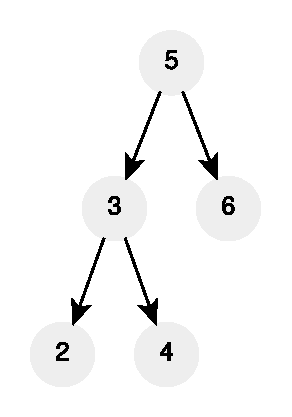
\includegraphics[width=\textwidth]{sources/next_greater_element_2/images/example1}
%	\caption[Sample short cpation]{Sample Caption}.
%	\label{fig:next_greater_element_2:example1}
%\end{figure}

\chapter{Next Greater Element \RN{2}}
\label{ch:next_greater_element_2}
\section*{Introduction}

\section{Problem statement}
\begin{exercise}
\label{example:next_greater_element_2:exercice1}
Write a function that  given a positive integer $n$, 
finds the smallest integer which:
\begin{itemize}
	\item it is greater in value than $n$
	\item has the exactly the same set of digits of $n$
	\item fits a $4$ bytes standard \inline{int},
\end{itemize} 
If no such positive integer exists, the function returns $-1$.
 
	%example1
	\begin{example}
		\label{example:next_greater_element_2:example1}
		\hfill \\
		Given $n=12$ the function returns $21$.
	\end{example}

	%example2
	\begin{example}
		\label{example:next_greater_element_2:example2}
		\hfill \\
		Given $n=21$ the function returns $-1$. No number can be composed with the digits $1$ and $2$ that 
		is greater than $21$.
	\end{example}

	\begin{example}
		\hfill \\
		Given $n = 778947$ the function returns $778974$.
	\label{ex:next_greater_element_2:example3}
	\end{example}
\end{exercise}

\section{Clarification Questions}

\begin{QandA}
	\item 
	\begin{answered}
		\textit{}
	\end{answered}
	
\end{QandA}

\section{Discussion}
\label{next_greater_element_2:sec:discussion}


\subsection{Brute-force}
\label{next_greater_element_2:sec:bruteforce}

\begin{minipage}{\linewidth}
	\lstinputlisting[language=c++, caption={Sample Caption},label=list:next_greater_element_2]{sources/next_greater_element_2/next_greater_element_2_solution1.cpp}
\end{minipage}

